% A skeleton file for producing Computer Engineering reports
% https://kgcoe-git.rit.edu/jgm6496/KGCOEReport_template

\documentclass[CMPE]{KGCOEReport}

% The following should be changed to represent your personal information
\newcommand{\classCode}{CMPE 160}  % 4 char code with number
\newcommand{\name}{Andrei Tumbar}
\newcommand{\LabSectionNum}{4}
\newcommand{\LabInstructor}{Mr.\ Byers}	% The slash is to tell LaTeX that the period is between words
												% not sentences so it spaces correctly. It won't appear in the
												% final pdf
\newcommand{\TAs}{Sam Myers \\ Kobe Balin \\ Georgi Thomas}
\newcommand{\LectureSectionNum}{1}
\newcommand{\LectureInstructor}{Mr.\ Cliver}
\newcommand{\exerciseNumber}{8}
\newcommand{\exerciseDescription}{Analysis and Simulation of Sequential Circuits}
\newcommand{\dateDone}{March 26th}
\newcommand{\dateSubmitted}{April 2th}

\graphicspath{{./lab8_media/}}

\usepackage{circuitikz}
\usepackage{tikz}
\usepackage{multirow}
\usepackage{titlesec}
\usepackage{float}
\usepackage{pgfplots, pgfplotstable}
\usepackage{lmodern}
\usepackage{siunitx}
\usepackage{subcaption}

\usepackage[usestackEOL]{stackengine}
\usepackage{scalerel}

\usepackage{kmap}
\usepackage[T1]{fontenc}

\usepackage{amsmath}

\def\lbar#1{\ThisStyle{%
  \setbox0=\hbox{$\SavedStyle#1$}%
  \stackengine{2.2\LMpt}{$\SavedStyle#1$}{\rule{\wd0}{0.1\LMpt}}{O}{c}{F}{F}{S}%
}}

\ctikzset{bipoles/not port/circle width=.4}
\ctikzset{tripoles/american xor port/height/.initial=.4}
\ctikzset{tripoles/american xor port/width/.initial=.6}

\DeclareFontFamily{U}{mathx}{\hyphenchar\font45}
\DeclareFontShape{U}{mathx}{m}{n}{ <-> mathx10 }{}
\DeclareSymbolFont{mathx}{U}{mathx}{m}{n}
\DeclareFontSubstitution{U}{mathx}{m}{n}
\DeclareMathAccent{\widebar}{\mathalpha}{mathx}{"73}

\makeatletter
\newcommand{\cwidebar}[2][0]{{\mathpalette\@cwidebar{{#1}{#2}}}}
\newcommand{\@cwidebar}[2]{\@cwideb@r{#1}#2}
\newcommand{\@cwideb@r}[3]{%
  \sbox\z@{$\m@th\mkern-#2mu#3\mkern#2mu$}%
  \widebar{\box\z@}%
}
\makeatother

\begin{document}
\maketitle

\section*{Abstract}

In the laboratory exercise a 4-bit shift register was created using four D flip-flops. The circuit had the ability to load a serial input into the shift register or to perform a parallel load of the four bits. After every clock, the bits where shifted through the flip-flops. A circuit was implemented and simulated using AOI logic and later converted to tri-state buffers for simplicity.

\section*{Design Methodology}

The shift register must be able to set the values of $Q_A$, $Q_B$, $Q_C$, and $Q_D$ synchronously (on the clock-edge) and also to shift the value of the four-bit number synchronously. This functionality is decided by the value of the \texttt{SL} or select pin. When this pin is \texttt{HIGH}, the values in the four bit register are set to $A$, $B$, $C$, and $D$ on the next rising clock edge. Otherwise, when the select pin is \texttt{LOW}, the shift register will shift the four bit number and $Q_A$ will take the value of the serial pin (\texttt{SIN}). The final functionality of this circuit is to reset the value of every flip-flop asynchronously. This can be achieved using the active-low asynchronous resets on every D flip-flop. 

\begin{table}[h!]
\renewcommand{\arraystretch}{1.2}
\setlength{\tabcolsep}{12pt}
\caption{Function table for 4-bit shift register.}
\begin{center}
\begin{tabular}{|c|c|c||c|c|c|c|l}
\cline{1-7}
\texttt{CLK} & \texttt{RST} & \texttt{SL} & ${Q_A}^*$ & ${Q_B}^*$ & ${Q_C}^*$ & ${Q_D}^*$ & \\\cline{1-7}
X & 0 & X & 0 & 0 & 0 & 0 & reset \\\cline{1-7}
$\uparrow$ & 1 & 0 & \texttt{SIN} & $Q_A$ & $Q_B$ & $Q_C$ & shift \\\cline{1-7}
$\uparrow$ & 1 & 1 & A & B & C & D & load \\\cline{1-7}
not rising & 1 & X & $Q_A$ & $Q_B$ & $Q_C$ & $Q_D$ & hold \\\cline{1-7}
\end{tabular}
\end{center}
\label{tab:func}
\end{table}

Table \ref{tab:func} shows all of the possible actions that can be performed on this circuit. The first of which is the asyncronous reset which does not rely on any particular value of the clock and will not be affected by the value of the select pin. The shift action will make the next value of each flip-flop (denoted by the *), to be the value of the previous bit. The first flip-flop will take on the value of the serial input. This action will only be performed when the clock edge is rising. The load action will also only occur on the rising clock edge and will take on the values of the parallel input pins, $A$, $B$, $C$, and $D$. Finally, the hold action will occur when the reset is not \texttt{LOW} and the clock edge is not rising. This will merely keep the current value of each D flip-flop.\\


The circuit was then implemented in Quartus using the D flip-flop component.

\pagebreak

\begin{figure}[h!]
	\centering
	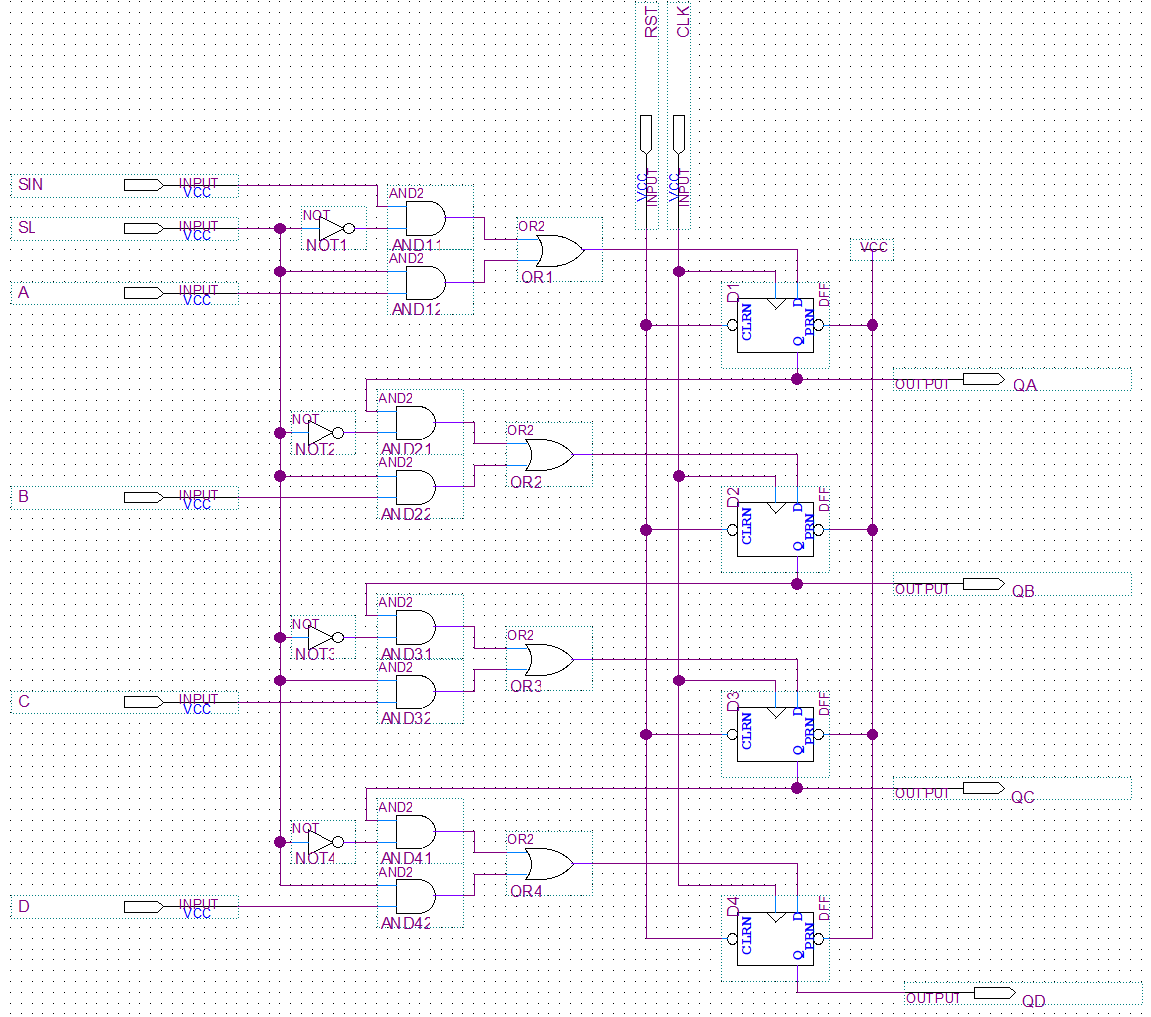
\includegraphics[height=12cm]{schematic1}
	\caption{4-bit shift register circuit schematic}
	\label{fig:shift-schem-aoi}
\end{figure}

Figure \ref{fig:shift-schem-aoi} is a circuit schematic of the 4-bit shift register described in Table \ref{tab:func}. The AOI logic that feeds into the \texttt{D} value of each flip-flop will determine whether to shift the register or to load it.\\

\pagebreak

The AOI logic can be further simplified using a new component call a tri-state buffer. The tri-state buffer is an useful tool in circuit design which allows a component of a circuit to disconnected electrically from the rest of a circuit. This use will become clear later.


\begin{figure}[h!]
	\centering
	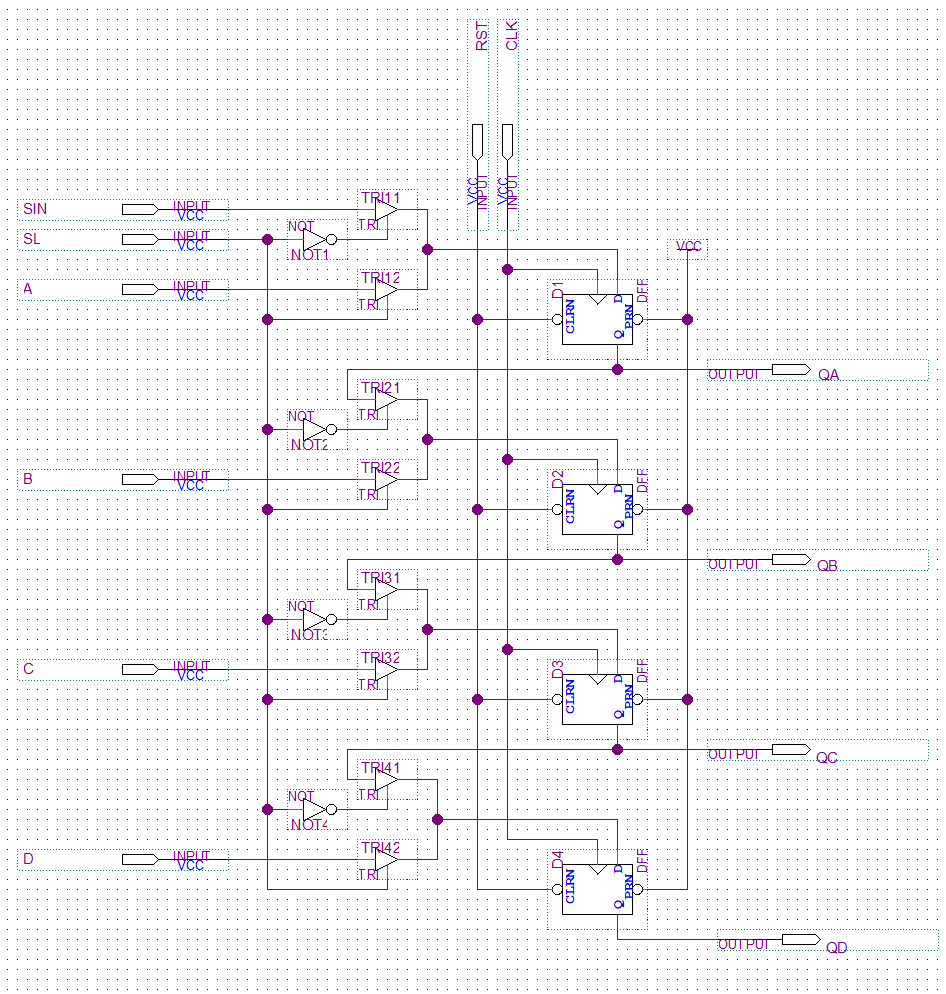
\includegraphics[height=12cm]{schematic2}
	\caption{4-bit shift register with tri-state buffers}
	\label{fig:shift-schem-tri}
\end{figure}

Figure \ref{fig:shift-schem-tri} shows the circuit schematic with the AOI logic feeding into the \texttt{D} inputs for each flip-flop changed to tri-state buffers. The tri-state buffer will take two inputs, a data input \texttt{A} and a control input which we will call the enable (\texttt{EN}). When the enable is \texttt{HIGH}, the output of the buffer will be logically equivalent to the input value, \texttt{A}. When the enable is \texttt{LOW}, the tri-state will yield a special output commonly refered to as \textbf{\emph{Hi-Z}}. In this state, the output is neither high or low but rather disconnected from the rest of the circuit. For example, when looking at the tri buffers going to the first D flip-flop in Figure \ref{fig:shift-schem-tri}, when the select is \texttt{LOW}, only the top buffer is enabled meaning that \texttt{D} is only wired to the \texttt{SIN} pin and the \texttt{A} pin is effectively disconnected. This is another way to implement a 2-1 mux with the select pin as an input and \texttt{SIN} and \texttt{A} being select lines.

\section*{Results and Analysis}

The two Quartus models were simulated in Modelsim to produce a waveform with all of the relative input and output signals. The input signals were defined using the following criteria:

\begin{itemize}
\item Reset before the first clock cycle.
\item Clock Cycle 1: parallel load of the number $B_{16}$ (hex) to the register
\item Clock Cycles 2-3: shift right two times while serial input is equal to 0.
\item Clock Cycles 4-5: shift right two times while serial input is equal to 1.
\end{itemize}

\begin{figure}[h!]
	\centering
	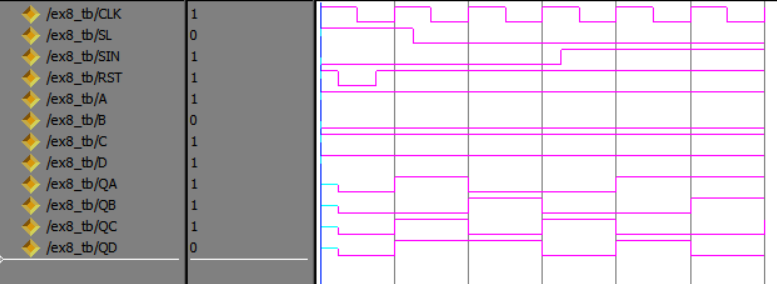
\includegraphics[width=\textwidth]{serial_shift.png}
	\caption{Shift register simulation wave capture.}
	\label{fig:reg-sim}
\end{figure}

Figure \ref{fig:reg-sim} shows the results of the a modelsim simulation run with the 4-bit shift register circuit. Both the diagrams from Figures \ref{fig:shift-schem-aoi} and \ref{fig:shift-schem-tri} yielded the same waveforms because they are just different implementations of the same circuit.\\

When looking at the timing of a circuit that includes a clock, one must examine the minimum clock period or the maximum clock frequency. This is an important classification to ensure the integrity of the outputs. There are times before and after the clock edge where a change in the D inputs should not change. These periods are called setup and clock to output times denoted by $t_s$ and $t_{co}$ respectively. The final time period that causes a delay is the propagation delay from the circuit logic denoted by $t_pd$. The following equation could be extracted from quartus after designing the circuit.

\begin{align}
\label{eq:reg}
T_{min} = t_{co} + t_{pd} + t_s = 5.809\,ns + 0\,ns + 2.201\,ns = 8.1\,ns \\
f_{max} = \frac{1}{T_{min}} = \frac{1}{8.1 \cdot 10^{-6}} = 123.4\,Mhz
\end{align}

The minimum clock period and the maximum frequency were calculated to be $8.1\,ns$ and $123.4\,Mhz$ respectively. If these limits are exceeded the output of the circuit is undefined because a insufficient amount of time is allowed before and after the clock edge to provide a meaningful output.

\section*{Conclusion}

In this laboratory exercise, a 4-bit shift register with parallel load and asynchronous reset was implemented in quartus and simulated in Modelsim. The lab was looking to provide more insight on the functionality of a serial loader and to also expose the idea of the tri-state buffer. This exercise was successful in doing so as it provided a comprehensive shift register example.

\section*{Questions}

\begin{enumerate}

\item A right bit shift operation with a zero introduced for the most significant bit is the same as performing an integer division by two.

\item A left bit shift with a zero introduced in the least significant bit is the same as multiplying by two.

\item If the input signal of a flip-flop is changed on the rising clock edge, the output is undefined because there is no way of knowing if the flip-flop looked at the value before or after the change.

\end{enumerate}
\end{document}
